\chapter{Конструкторская часть}

В данном разделе будут рассмотрены схемы алгоритмов сортировок 
(блинная, перемешиванием и пирамидальная), а также найдена их трудоемкость.

\section{Разработка алгоритмов}

\begin{figure}[h]
    \centering
    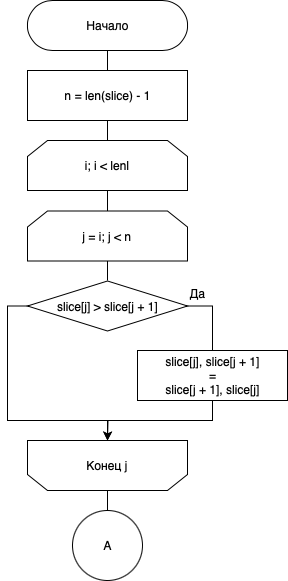
\includegraphics[width=0.4\linewidth]{img/sheker1.jpg}
    \caption{Схема алгоритма сортировки Перемешиванем}
    \label{fig:shecker}
\end{figure}

\begin{figure}[h]
    \centering
    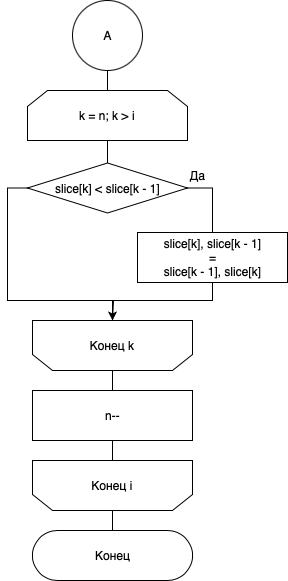
\includegraphics[width=0.4\linewidth]{img/sheker2.jpg}
    \caption{Схема алгоритма сортировки Перемешиванем}
    % \label{fig:shecker}
\end{figure}

\begin{figure}[h]
    \centering
    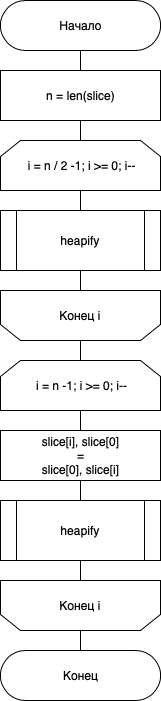
\includegraphics[width=0.2\linewidth]{img/piramid1.jpg}
    \caption{Схема алгоритма Пирамидальной сортировки. Основная функция.}
    % \label{fig:shecker}
\end{figure}

\begin{figure}[h]
    \centering
    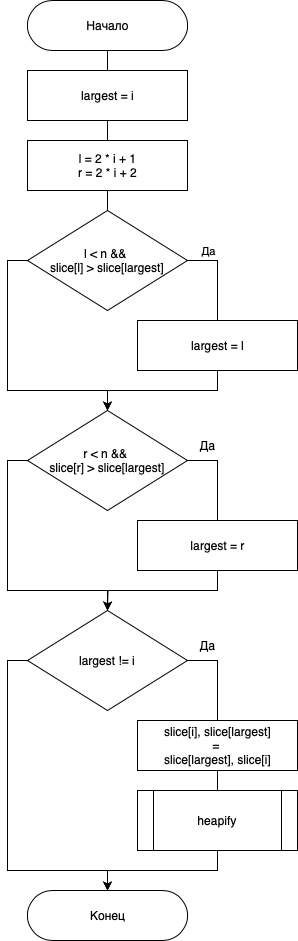
\includegraphics[width=0.4\linewidth]{img/piramid2.jpg}
    \caption{Схема алгоритма Пирамидальной сортировки. Функция поиска максимального.}
    % \label{fig:shecker}
\end{figure}



